\documentclass[11pt,article]{memoir}
%Layout
	\usepackage[a4paper,left=3.5cm, right=3.5cm, top=3cm, bottom=3cm]{geometry}
	\usepackage{authblk}
	\usepackage{rotating}
	\DisemulatePackage{setspace}
	\usepackage{setspace}
	\onehalfspacing
	\counterwithout{section}{chapter}
	\usepackage[hang,small,bf]{caption}
	\setcounter{secnumdepth}{2}
%Fonts and encoding
	\usepackage{amsfonts}
	\usepackage{amssymb}
	\usepackage{amsmath}
	\usepackage{bm}
	\usepackage[T1]{fontenc}
	\usepackage[utf8]{inputenc}
	%\usepackage{lmodern}
	%\usepackage{fouriernc}
%Graphics and tables
	\usepackage{graphicx}
	\usepackage{placeins}
	\usepackage{tabularx,booktabs}
	\usepackage{longtable}
	\usepackage{subfig}
	\usepackage{rotating}
	\usepackage{array,multirow}
	\usepackage{threeparttable}
 \usepackage[]{endfloat}
%References
	\usepackage{natbib}
	\bibliographystyle{chicago}
% Handle Stata input    
    \newcommand{\sym}[1]{$^{#1}$}
		
%NJ extra
\makeatletter
\@fpsep\textheight
\makeatother	
\usepackage{csquotes}
\MakeOuterQuote{"}	
\setcounter{tocdepth}{3}
		
\title{How Useful are Posted Job Openings?\thanks{We are indepted to Paul Bingley, Per Krusell, Karsten Alb\ae k, John Hassler, Robert Shimer, Tobias Broer, Hannes Malmberg, Georg Marthin and Erik \"{O}berg for stimulating discussions and suggestions. We are very grateful to Charlotte Leolnar Reif, Anders Gabriel Pedersen, Klaus Henrik Langager and Charlotte Funk Christensen for providing us with data. All remaining errors are our own.}}



\author[1]{Niels-Jakob Harbo Hansen\thanks{Stockholm University, IIES.  Email: \texttt{nielsjakobharbo.hansen@iies.su.se}. Corresponding author. }}
\author[2]{Hans Henrik Sievertsen}

\affil[1]{Stockholm University, IIES}
\affil[2]{The Danish National Centre for Social Research (SFI)}

\date{Version: \today{}\\\emph{--- preliminary and incomplete version - please do not circulate ---}}
\begin{document}
\maketitle
\begin{abstract}
Policy makers and researchers often evaluate labor market efficiency using announced job openings and unemployment. It is well-known that announced job-openings  only constitute a fraction of all job openings in the economy, but less is known about how this fraction varies across time and firms. To inform this discussion we construct a new database with actual hires and announced job openings using data from the Danish tax authorities and Public Employment Service during 2004-2012. Using this we find that only 10-25 percent of all hires are made through announced hires, which via a simple model translates into 5-20 percent of all job openings being announced. We also find that the share of hires via announced openings being increasing in firm size, decreasing in employment growth, less used in start-ups than in existing firms and share exhibits an inverse u-shape in the firm' average wage level. Second, we set up and calibrate a simple search-and-matching model with two recruitment channels: announced and unannounced job openings. Using this model we show how the observed swings in the fraction of posted job openings significantly influences the perceived matching efficiency and Beveridge curve movements.
\end{abstract}  

\newpage

\section{Introduction}

Job openings is a key component in labor market analysis within the search matching framework. In the canonical search matching model (\emph{e.g.} as presented in \cite{Pissarides2000}) hires happens as unemployed workers and job openings created by firms meet via an aggregate matching function. The success of this framework stems from its ability to match the observed labor market behaviour over the business cycles. Indeed, in the model a positive productivity shock will increase the firms' payoff from a match and thus induce it to create more job openings. As the labor market becomes tighter hiring increases and unemployment falls. %That is, the economy moves along the Beveridge curve.

Thus, time series for job openings are key when taking the model to the data. Unfortunately, our understanding of job openings is far from full. On a conceptual level the economic content of a job opening is not clear,\footnote{\citet{Abraham1983} defines a job opening as unmet labor demand, but \cite{Elsby2014} suggest this definition could be misleading as (1) while it relatively straightforward to  identify a idle worker it is less so to identify idle resources at the firm level, (2) it is difficult to identify the amount of desired production not being undertaken due to an unfilled opening and (3) firms might choose to recruit for positions in anticipate of these being opened in the future.} and there are also serious challenges in measurement. Indeed, time series for job openings are often based on postings in media or at public employment services. An obvious concern is that postings via these channels are not representative for all openings, and that the firm's propensity to use these channels can vary over time.\footnote{The establishment of the US Job Opening and Labor Turnover (JOLTS)Survey in December 2000 has eased these concerns. Instead of relying on job-postings JOLTS is a survey and defines a job openings as a position for which (i) work could start within $30$ days and (ii) the employer is \emph{actively recruiting} for outside the firm. However, the JOLTS only goes back to 2000 for the US and a similar surveys for Europe only exists from 2008.}

Not accounting for these measurement problems can lead to spurious conclusions within the search matching framework and ultimately to misguided policy. In the search matching framework movements in the Beveridge curve can only be caused by exogenous shifts in (i) the match efficiency or (ii) the job destruction rate. This observation has influenced the policy discussion in the wake of the Great Recession, where the Beveridge curve relation appears to have adversely shifted in both the United States and in Europe.\footnote{\emph{E.g.} The president of the European Central Bank, Mario Draghi, in his speech at Jackson Hole 2015 observed: \emph{"The euro area Beveridge curve [...] suggests the emergence of a structural mismatch across Euro area labor markets"} \citep{Draghi2014}. } However, as we will argue more precisely below shifts in the Beveridge curve can also be caused by change in firms recruitment behavior. Indeed, if firms substitute between observed postings and other channels this can also shift the Beveridge curve.\footnote{We are not new to make such a claim. Indeed, \cite{Davis2013} argue that changes in the \emph{recruitment intensity} of firms can shift the matching function.}

In this paper we use new Danish data and a simple theoretical framework in order to inform this discussion.
Specifically, we construct a database with firm level data on hires and job postings. Using this we compute the amount of announced and unannounced job openings and document how the share varies across time. We calibrate a simple search matching model to imitate this variation and show how this can create a shift in the perceived Beveridge curve.

We find that that only 10-25 percent of all hires during 2004-08 were made through announced openings. Using our model this translates into 5-20 percent of all job openings being announced. We find considerable variation in the use of announced openings across firm characteristics with the share of hires via announced openings being increasing in firm size, decreasing in employment growth and less used in start-ups than in existing firms. Moreover, the it exhibits an inverse u-shape in the average wage level of the firm with low and high wage firms relying the least on announced openings.  We also use our calibrated model to show how decrease in the share of announced hires from 20 to 10 percent leads to a 40 percent increase in the perceived matching efficiency.

Our paper relates to a number of papers in the literature. Most close in spirit is \cite{Davis2013} who analyzes hires and job-openings (JOLTS) in the US. They find that changes in the recruitment intensity of firms partly explains the recent breakdown in the standard matching function. Previously a vast literature has related the aggregate number of job-openings, unemployed and hires through the canonical search matching model (e.g. \cite{Blanchard1990}). Especially relevant from this literature strand are papers using job-openings from centralized registers \citep{Coles1996, Hansen2004, Yashiv2000, Sunde2007}. Also related is the literature that analyzes the determinants of job-opening durations \citep{Ours1991, Burdett1998, Barron1997, Holzer1990}.

The paper is organized as follows. Section \ref{sec:Data} presents our data and shows how hires with and without observed job-openings vary across time and worker characteristics. Section \ref{sec:model} sets up a search matching model with announced and unannounced job-openings which we use along with the data we back of the share of unannounced openings and assess the fluctuations in this share impact on the perceived matching efficiency. Section \ref{sec:conclusion} concludes and offers some thoughts on remaining work.

%\section{A Review of the Literature}
%\label{sec:litt}
%
%\begin{itemize}
	%\item A substantial literature on the behaviour of job-openings. A complete survey is beyond the scope of this text, but we refer to Elsby et al. (forthcoming).
	%\begin{itemize}
	%\item A early literature on the  help-wanted index for job-openings (Abraham, 1983; 1987). Abraham (1983) is relevant for our approach. She used data for new hires and average duration of openings in order to back out vacancy numbers.
	%\item Big literature which relates the aggregate number of job-openings and unemployed workers to number of hires (e.g. Blanchard and Diamond, 1989; Shimer, 2005; )
	%\item Especially relevant are studies using vacancy behaviour from centralized registers (Coles and Smith, 1996; Albaek and Hansen, 2004; Berman, 1997; Yashiv, 2000; Andrews, 2008; Sunde, 2007)
	%\item Also related is the literature which analyzes the duration of job-openings and their determinants (Ours and Ridder, 1991; Burdett and Cunningham, 1998; Barron et al., 1999; Holzer, 1990). 
	%\item But literature that relates job-openings to job hirs on the firm level is very scarce (Haltiwanger et al., 2013). 
	%\item TBD: Parallel with unemployment to job and job-to-job litterature.
	%\end{itemize} 
%\end{itemize}




\FloatBarrier
\section{Data and definitions}
\label{sec:Data}
We use data from four  sources: (1) Job Openings from the Public Employment Service. (2) The tax records for the entire Danish working population. (3) Administrative registers from Statistics Denmark. (4) Data on unemployment from Statistics Denmark.

 The job openings  dataset  contains all  vacancies announced at the Public Employment Service from 2004 to 2013. For each opening we have a firm identifier (CVRNR), the number of positions available, the day the opening was announced, and the day the announcement was withdrawn. For all firms in Denmark we have the tax records, that contains a firm identifier (CVRNR), a personal identifier (CPR),  the salary, and the first and last working day for each employee.  We use the data on the first and last day at work to construct the actual number of hires at each point in time. The administrative registers from Statistics Denmark provides information on all individuals demographics (gender, age, origin) and socio-economic background (education, employment type, income, wealth). The administrative registers also contain firm-level characteristics such as sector, size, and industry. 
 
%and covers approximately x percent of all job openings in Denmark \ref{}. 
\subsection{Definitions}
An \textit{announced job opening} is defined using the job openings dataset by the date the job posting was withdrawn, as this most likely is the last day the job seeker could apply for this job. We assess this assumption by collecting job postings from the online archive of the private provider "Jobindex.dk" of which the announcements at the public Employment Service is a subset. This data is useful as it contains data for the expected starting date and the date for withdrawal of the job posting. Figure \ref{fig:jobnet} shows the distribution of months from deadline to job starting date. For a considerably fraction of the announcements the job starting is set to as soon as possible (asap). Figure \ref{fig:jobnetb} shows that most non-asap postings have a job starting date within two months of the deadline. As a consequence we will evaluate the sensitivity of our analysis to setting the job starting day at three, two, one, or zero months after the deadline.

\begin{figure}[h!]
	\subfloat[Time to job start (all announcements)\label{fig:jobneta}]{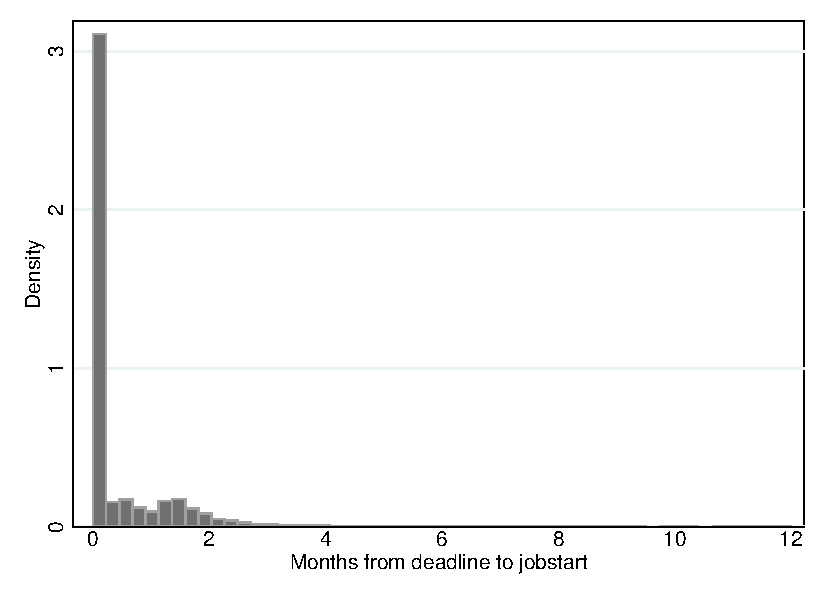
\includegraphics[width=.49\linewidth]{figures/time_to_start_all}}
	\subfloat[Time to job start (without asap)\label{fig:jobnetb}]{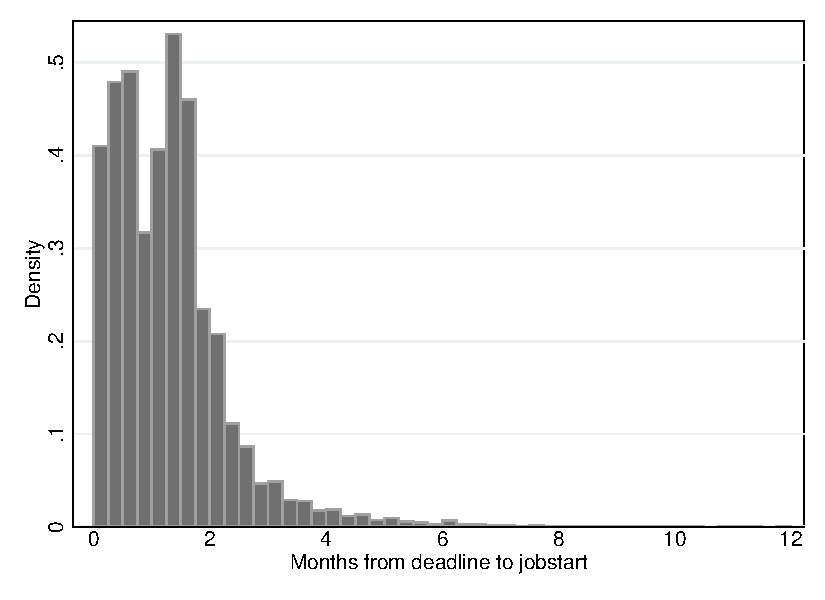
\includegraphics[width=.49\linewidth]{figures/time_to_start_all_without_asap}}
	\caption{Time to job start from deadline, measured in months. The data is collected from Jobindex.dk's online archive 2008-2014. In Figure \ref{fig:jobneta} the job start date of "as soon as possible" openings is sat equal the application deadline. In Figure \ref{fig:jobnetb} these job openings are removed.}
	\label{fig:jobnet}
\end{figure}

A \textit{job hire} is defined using the tax records. The hiring day is defined as the starting day of the an employment spell if the individual was not employed with the same firm in the previous 30 days.

For each job spell we define a new hire by the first working day of the year if the individual did not work at the same firm within 30 days before that hire. We only consider job hires where the job duration is more than 5 days. In 2008 the  271 municipalities in Denmark where merged to 99, and the 15 counties were replaced by five regions. A considerable number of public employees thus started working for a new employer on January 1st 2008. To separate these job starts from real job change, we use information from the Statistics Denmark on the year the employee started in the current job. For job-starts on January 1st 2008 we furthermore consider information on the firm size and the individual wage. If the individual was employed at a job in December 2011 with the same wage and/or firm size as the job start on January 1st, the new spell is not recorded as a new hire. 

An \emph{announced hire} is defined as a hire in a firm where an announced job-opening had deadline in same month. An \emph{unannounced hire} is defined as a hire where this is not the case. If $x$ hires are made in a firm with $y<x$ announced job-openings, then we count this as $y$ announced hires and $x-y$ unannounced hires. 

\subsection{Descriptives}

Figure \ref{fig:hires} show the monthly levels of annonuced job hires from 2004 to 2012. We notice that the level of unannounced hires is roughly an order of magnitude larger than the level of announced hires. Both curves display business cycle movements, but the movements are stronger for announced hires. Figure \ref{fig:hires_shares} display the time serie for the share of announced hires out of total. This shows that announced hires account for TBD-TBD percent of all hires. The share displays a clear pro-cyclical pattern.

\begin{figure}[h]
\begin{center}
		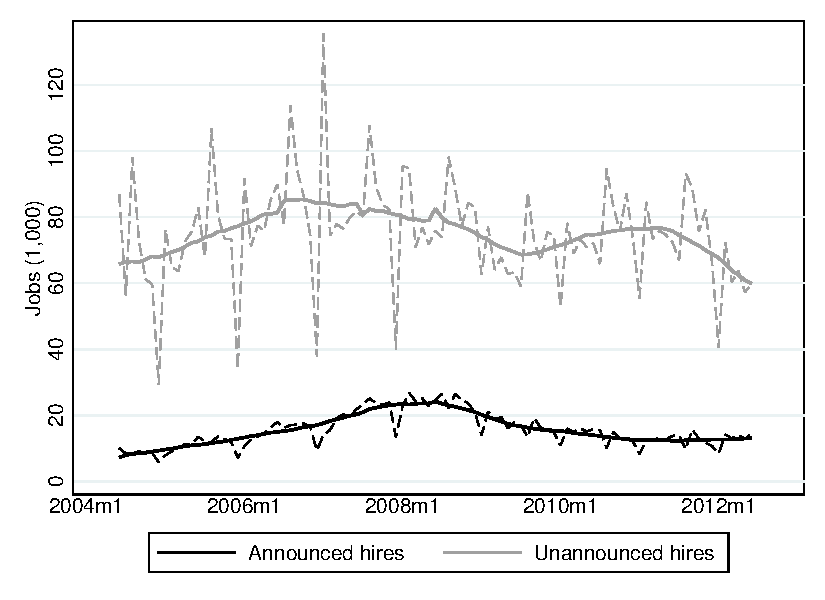
\includegraphics[width=.98\linewidth]{figures/overview_full}
	\caption{Hires through announced and unannounced positions. The dashed lines indicate the unadjusted monthly levels, the solid lines are six month moving average (with equal weights). }
	\label{fig:hires}
\end{center}
\end{figure}

\begin{figure}[h]
\begin{center}
		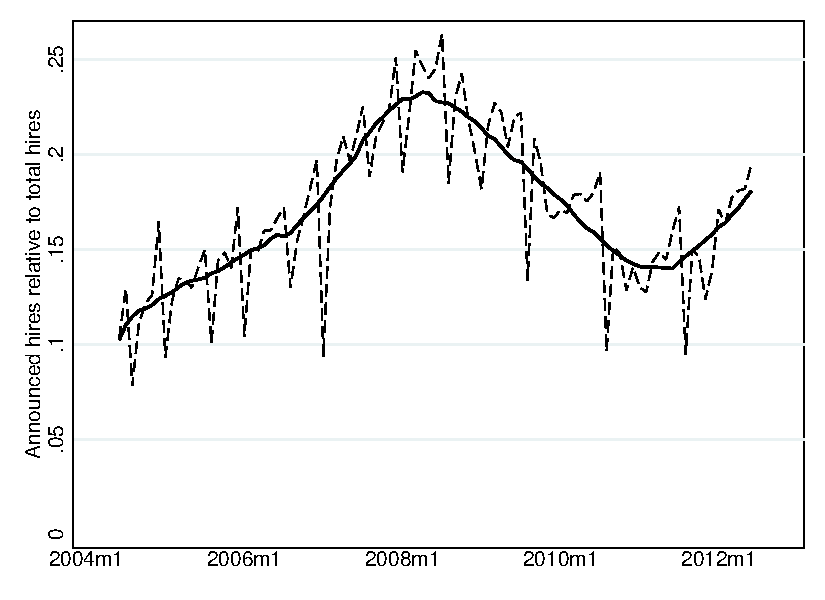
\includegraphics[width=.98\linewidth]{figures/overview_rate_HAHT}
	\caption{The share of announced hires out of total hires. The dashed lines indicate the unadjusted monthly levels, the solid lines are six month moving average (with equal weights). }
	\label{fig:hires_shares}
\end{center}
\end{figure}

Table \ref{tab:maindesc} provides monthly means for the key variables. The first row gives the average for the full population. A firm had on average 3.5 hires per month, but only 0.6 of these hires were through an announced opening. The average firm size is 18 full year employees. 

%Panel A in Table \ref{tab:maindesc} shows that the total number of hires is increasing in the firms average wage, but non-monotonically as the 60-80th quantile has the highest number of hires with 5 hires per month. It is also worth noting that the firm size is increasing in wage.\footnote{The firms' average wage is calculated by using length of employment spell and total salary from the individual tax records to compute the average salary per day employed. For each firm we then compute the weighted average, where the individual is weighted by the length of the employment spell, such that the average wage of the individual who is employed for six months has a larger weight than the wage of the individual who was employed for three months. The wage deciles are then calculated separately for each year. }

Jobs in the public sector are more often matched through announced vacancies than jobs in the private sector, as shown by Panel B in Table \ref{tab:maindesc}. These public workplaces are  larger on average, which might explain why larger workplaces hire relatively more workers through announced vacancies as shown from the numbers in Panel C. %Another relevant factor is that the public sector is required to recruit via public job openings.

Table \ref{tab:size} presents the ratio of announced to total number of hires by firm size for each year 2004 to 2012. In general, the ratio is increasing in firm size, but the slope of the increase is considerably smaller in the post 2008 years. 

Panel C shows that the use of announced hires is increasing the firm size, which is further illustrated in Table \ref{tab:size} where the ratio of announced to total hires is shown for each year from 2004-12. 
Panel D shows that startups are less reliant on announced openings than existing firms, and Table \ref{tab:growth} shows that the ratio is decreasing in firms' employment growth in each year. Finally, Panel E shows substantial differences in recruiting behaviour across industries, with \emph{manufacturing} relying most on announced openings and \emph{energy} relying least.

\begin{table}[h!]
	\caption{Statistics by firm characteristics - monthly averages 2004-2012}
	\label{tab:maindesc}
	\begin{tabularx}{\linewidth}{cXcccccr}
	\toprule[1pt]
	&&HT&OA&HA&HU&HA/HT&Size\\
	\midrule
		&All& 3.49& 1.08& 0.58& 2.91& 0.06&18.01\\
\multicolumn{7}{l}{\textit{By wage decile}}\\
&0-20\% (lowest)& 2.25& 0.51& 0.16& 2.08& 0.04& 3.81\\
&20-40\%& 2.81& 0.70& 0.31& 2.50& 0.06& 8.19\\
&40-60\%& 3.93& 1.23& 0.76& 3.17& 0.06&13.06\\
&60-80\%& 4.94& 2.01& 1.30& 3.64& 0.07&25.07\\
&80-100\% (highest)& 4.00& 1.22& 0.55& 3.44& 0.06&40.61\\
\multicolumn{7}{l}{\textit{By sector}}\\
&Unknown& 3.55& 1.11& 0.53& 3.03& 0.07&19.52\\
&Central government& 5.96& 1.57& 1.10& 4.85& 0.08&27.80\\
&Regional government&13.42& 7.53& 6.04& 7.38& 0.09&24.52\\
&Municipalities&11.00& 6.67& 5.08& 5.92& 0.11&18.42\\
&Public companies&40.35&27.11&20.79&19.56& 0.23&65.77\\
&Private secor& 2.66& 0.59& 0.25& 2.40& 0.04&15.59\\
\multicolumn{7}{l}{\textit{By firm size (\# of employees)}}\\
&2-3& 2.30& 0.61& 0.31& 1.99& 0.03& 2.37\\
&3-4& 2.57& 0.82& 0.40& 2.17& 0.05& 3.72\\
&5-9& 3.18& 0.88& 0.48& 2.69& 0.06& 6.95\\
&10-19& 3.89& 1.33& 0.76& 3.13& 0.07&13.92\\
&20-49& 4.46& 1.52& 0.81& 3.66& 0.09&30.56\\
&>49& 9.70& 3.30& 2.01& 7.70& 0.12&130.20\\
\multicolumn{7}{l}{\textit{By firm growth (year-to-year change in \# of employees)}}\\
&New firm& 2.17& 0.43& 0.14& 2.03& 0.03& 2.68\\
&<-10\%& 5.34& 2.00& 1.19& 4.16& 0.07&11.77\\
&-10-0\%& 2.48& 0.54& 0.26& 2.22& 0.06&28.25\\
&0\%& 1.89& 0.40& 0.17& 1.73& 0.05& 7.66\\
&0-10\%& 2.64& 0.57& 0.25& 2.39& 0.06&32.43\\
&10-25\%& 2.56& 0.67& 0.32& 2.23& 0.06&21.38\\
&>25\%& 4.99& 1.81& 1.04& 3.95& 0.07&20.73\\
\multicolumn{7}{l}{\textit{By industry}}\\
&Construction& 1.90& 0.47& 0.16& 1.74& 0.06&16.92\\
&Energy& 2.88& 0.22& 0.11& 2.77& 0.03&44.50\\
&Finance& 4.32& 2.69& 1.02& 3.29& 0.07&20.04\\
&Trade, hotel \& restaurants& 2.73& 0.70& 0.35& 2.38& 0.08&13.49\\
&Manufactoring& 3.03& 0.98& 0.43& 2.60& 0.10&47.91\\
&Farms, ?sheries \& mining& 2.39& 0.40& 0.19& 2.20& 0.06&37.07\\
&Public \& private services& 7.00& 1.73& 1.07& 5.93& 0.07&21.28\\
&Transportation, mail and com. & 3.59& 1.00& 0.45& 3.14& 0.07&22.66\\
&Unknown& 1.40& 0.08& 0.03& 1.36& 0.02& 0.87\\

		\bottomrule[1pt]
	\end{tabularx}
	\begin{minipage}{\linewidth}
		\footnotesize{Notes: HT: Total number of hires. OA: Number of announced vacancies. HA: Number of hires related to an announced vacancy. HU: number of hires without a post vacancy. HA/HT: Hires through vacancies in relation to the total number of hires. Size: firm size (by the number of employees.). Sector is only known for 2008-2012.}
	\end{minipage}
\end{table}

Figure \ref{fig:WD} shows the ratio of announced to total number of hires by wage decile.\footnote{The firms' average wage is calculated by using length of employment spell and total salary from the individual tax records to compute the average salary per day employed. For each firm we then compute the weighted average, where the individual is weighted by the length of the employment spell, such that the average wage of the individual who is employed for six months has a larger weight than the wage of the individual who was employed for three months. The wage deciles are then calculated separately for each year. } 
Figure \ref{fig:WD1} covers the full period and shows a clear reverse U-shape. The lowest and highest deciles have the lowest rate of announced hires. Figure \ref{fig:WD2}  provides a pre- to post 2008  comparison of the ration of announced to total number of hires by wage deciles. For both periods we see a clear reverse U-shape, but the level considerably lower after 2008. 

% \begin{table}[h!]
% 	\caption{The ratio of announced hires to total hires, by wage decile 2004-2012}
% 	\label{tab:wagedecile}
% 	\begin{tabularx}{\linewidth}{X|cccccccccc}
% 	\toprule[1pt]
% 	&\multicolumn{10}{c}{- - -  Wage Decile - - -}\\
% 	&	1.&	2.&	3.&	4.&	5.&	6.&	7.&	8.&	9.&	10.\\\midrule
% 		2004&0.044&0.027&0.046&0.051&0.052&0.058&0.063&0.067&0.069&0.044\\
2005&0.051&0.031&0.064&0.067&0.064&0.078&0.080&0.092&0.095&0.056\\
2006&0.070&0.038&0.079&0.078&0.082&0.088&0.102&0.108&0.114&0.064\\
2007&0.069&0.042&0.078&0.080&0.082&0.098&0.095&0.100&0.094&0.055\\
2008&0.058&0.023&0.068&0.079&0.076&0.088&0.090&0.097&0.089&0.037\\
2009&0.043&0.019&0.053&0.055&0.053&0.048&0.064&0.053&0.051&0.028\\
2010&0.043&0.021&0.050&0.052&0.043&0.043&0.052&0.047&0.048&0.024\\
2011&0.042&0.020&0.046&0.047&0.041&0.050&0.050&0.050&0.048&0.026\\
2012&0.047&0.023&0.050&0.049&0.050&0.057&0.052&0.056&0.053&0.035\\

% 		\bottomrule[1pt]
% 	\end{tabularx}
% \end{table}

\begin{figure}[h!]
	\subfloat[All years \label{fig:WD1}]{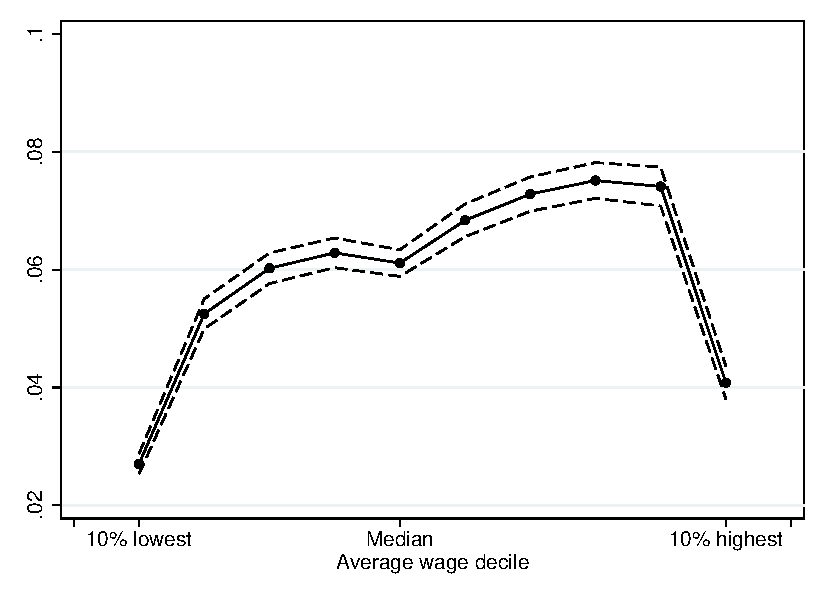
\includegraphics[width=.49\linewidth]{figures/plot_cross_sec_wagedecile}}
	\subfloat[Pre-Post 2008 \label{fig:WD2}]{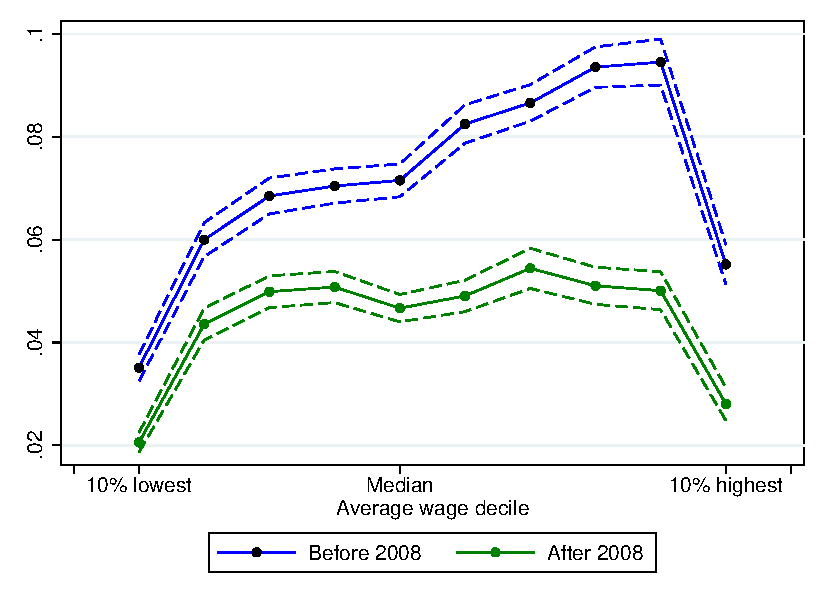
\includegraphics[width=.49\linewidth]{figures/plot_cross_sec_wagedecile_bef2008}}
	\caption{The ratio of announced hires to total hires by wage decile. The wage is the average wage in the firm. }
	\label{fig:WD}
\end{figure}

% \begin{table}[h!]
% 	\caption{The ratio of announced hires to total hires, by industry 2004-2012}
% 	\label{tab:industry}
% 	\begin{tabularx}{\linewidth}{Xr}
% 	\toprule
% 		&Construction& 0.05&17.03\\
&Energy& 0.03&47.64\\
&Finance& 0.06&20.54\\
&Trade, hotel and restaurants& 0.06&13.48\\
&Manufacturing& 0.08&48.52\\
&Farms, fisheries and raw materials& 0.05&37.64\\
&Public and private services& 0.05&21.23\\
&Transportation, mail and communications& 0.05&22.83\\
&Unknown& 0.02& 0.92\\

% 		\bottomrule
% 	\end{tabularx}
% \end{table}





% \begin{table}[h!]

\begin{table}[h!]
\begin{center}
		\caption{The ratio of announced hires to total hires, by firm size 2004-2012}
	\label{tab:size}
	\begin{tabularx}{.65\linewidth}{X|cccccc}
	\toprule
	&\multicolumn{6}{c}{\# Employees (full year equ.)}\\
	&<3&3-4&5-9&10-19&20-49&>50\\\midrule
		2004&0.029&0.040&0.048&0.056&0.076&0.101\\
2005&0.041&0.051&0.059&0.077&0.097&0.138\\
2006&0.051&0.063&0.072&0.094&0.119&0.168\\
2007&0.046&0.061&0.074&0.095&0.115&0.155\\
2008&0.034&0.060&0.070&0.095&0.113&0.156\\
2009&0.025&0.039&0.049&0.064&0.068&0.100\\
2010&0.024&0.036&0.046&0.056&0.060&0.086\\
2011&0.024&0.035&0.046&0.055&0.059&0.084\\
2012&0.028&0.037&0.045&0.059&0.065&0.087\\

		\bottomrule
	\end{tabularx}
\end{center}
\end{table}


\begin{table}[h!]
\begin{center}
		\caption{The ratio of announced hires to total hires, by firm growth 2004-2012}
	\label{tab:growth}
	\begin{tabularx}{.85\linewidth}{X|cccccc}
	\toprule
	&\multicolumn{6}{c}{Growth in \# Employees (full year equ.)}\\
	&<-10\%&10-0\%&No change&0-10\%&10-25\%&>25\%\\\midrule
		2004&0.065&0.071&0.037&0.074&0.052&0.058\\
2005&0.084&0.095&0.049&0.097&0.074&0.075\\
2006&0.101&0.112&0.059&0.121&0.096&0.089\\
2007&0.096&0.107&0.057&0.114&0.094&0.090\\
2008&0.085&0.079&0.071&0.074&0.067&0.082\\
2009&0.049&0.042&0.021&0.047&0.046&0.057\\
2010&0.047&0.037&0.053&0.039&0.042&0.051\\
2011&0.047&0.038&0.075&0.040&0.035&0.052\\
2012&0.054&0.040&0.024&0.042&0.041&0.053\\

		\bottomrule
	\end{tabularx}
\end{center}
\end{table}



%\begin{itemize}
	%\item Variation by firm characteristics 
	%
	%\begin{center}
	%[Insert table with share announced hires per sector]
	%
	%\end{center}
	%
	%\item Variation by worker characteristics. Here we focus on hires where it can be identified whether the hire done via an announced opening or not.
	%
	%\begin{center}
	%[Insert table with share announced hire by education] 
	%
  %[Insert table with share announced hire by status before hire ] 
	%
	%[...]
	%\end{center}
%\end{itemize}

\section{The Model}
\label{sec:model}
In this section we set up a simple search-matching model of the labor market. The model builds heavily on the framework by the canonical model laid out in \cite{Pissarides2000}. However,  in line with the empirical analysis above we will allow firms and workers to match via two channels: announced and unannounced job-openings. An announced opening is a ordinary job vacancy posting, visible for labor market analysts. An unannounced opening is a opening that is not posted publicly, but where the firm instead relies on alternative recruiting channels such as uninvited applications or networks. The only heterogeneity between announced and unannounced job openings will be differences in the cost of posting.

The purpose of this model is twofold. First, we wish to illustrate how changes in the posting behavior of firms can shift the \emph{perceived} matching efficiency in the economy. Second, we construct a framework that empirically will allow us to trace out the shared of announced and unannounced job openings in the economy (Section \ref{sec:Cali}). 

\subsection{The model}


\subsubsection{The Matching Functions}

A non-standard element in our model will be the existence of two matching function - each with one type of job-openings. Unemployed search on both markets, while firms will only post a fraction of all their openings (see below). Specifically, unemployed workers and announced openings are matched according to the function
\begin{align}
M_A \left( U, O_A \right)= A U ^\alpha O_A^{ 1-\alpha }
\label{eq:M_A}
\end{align}
while unemployed and unannonced openings are matched according to 
\begin{align}
M_U \left( U, O_A \right)= A U ^\alpha O_U^{ 1-\alpha } 
\label{eq:M_U}
\end{align}

It follows that the probability of filling an announced opening is $m_A(\theta) \equiv \frac{M_A \left( U, O_A \right)}{O_A}$, where $\theta=\frac{O_A}{U}$, while the probability for a unemployed to match into a announced opening is $\theta m_A(\theta)$. Similarly, the probability of filling an unannounced opening is $m_U (\kappa)$, where $\kappa=\frac{O_U}{U}$,  while the chance for an unemployed to matching in to such a position is $\kappa m_U (\kappa)$.

\begin{figure}
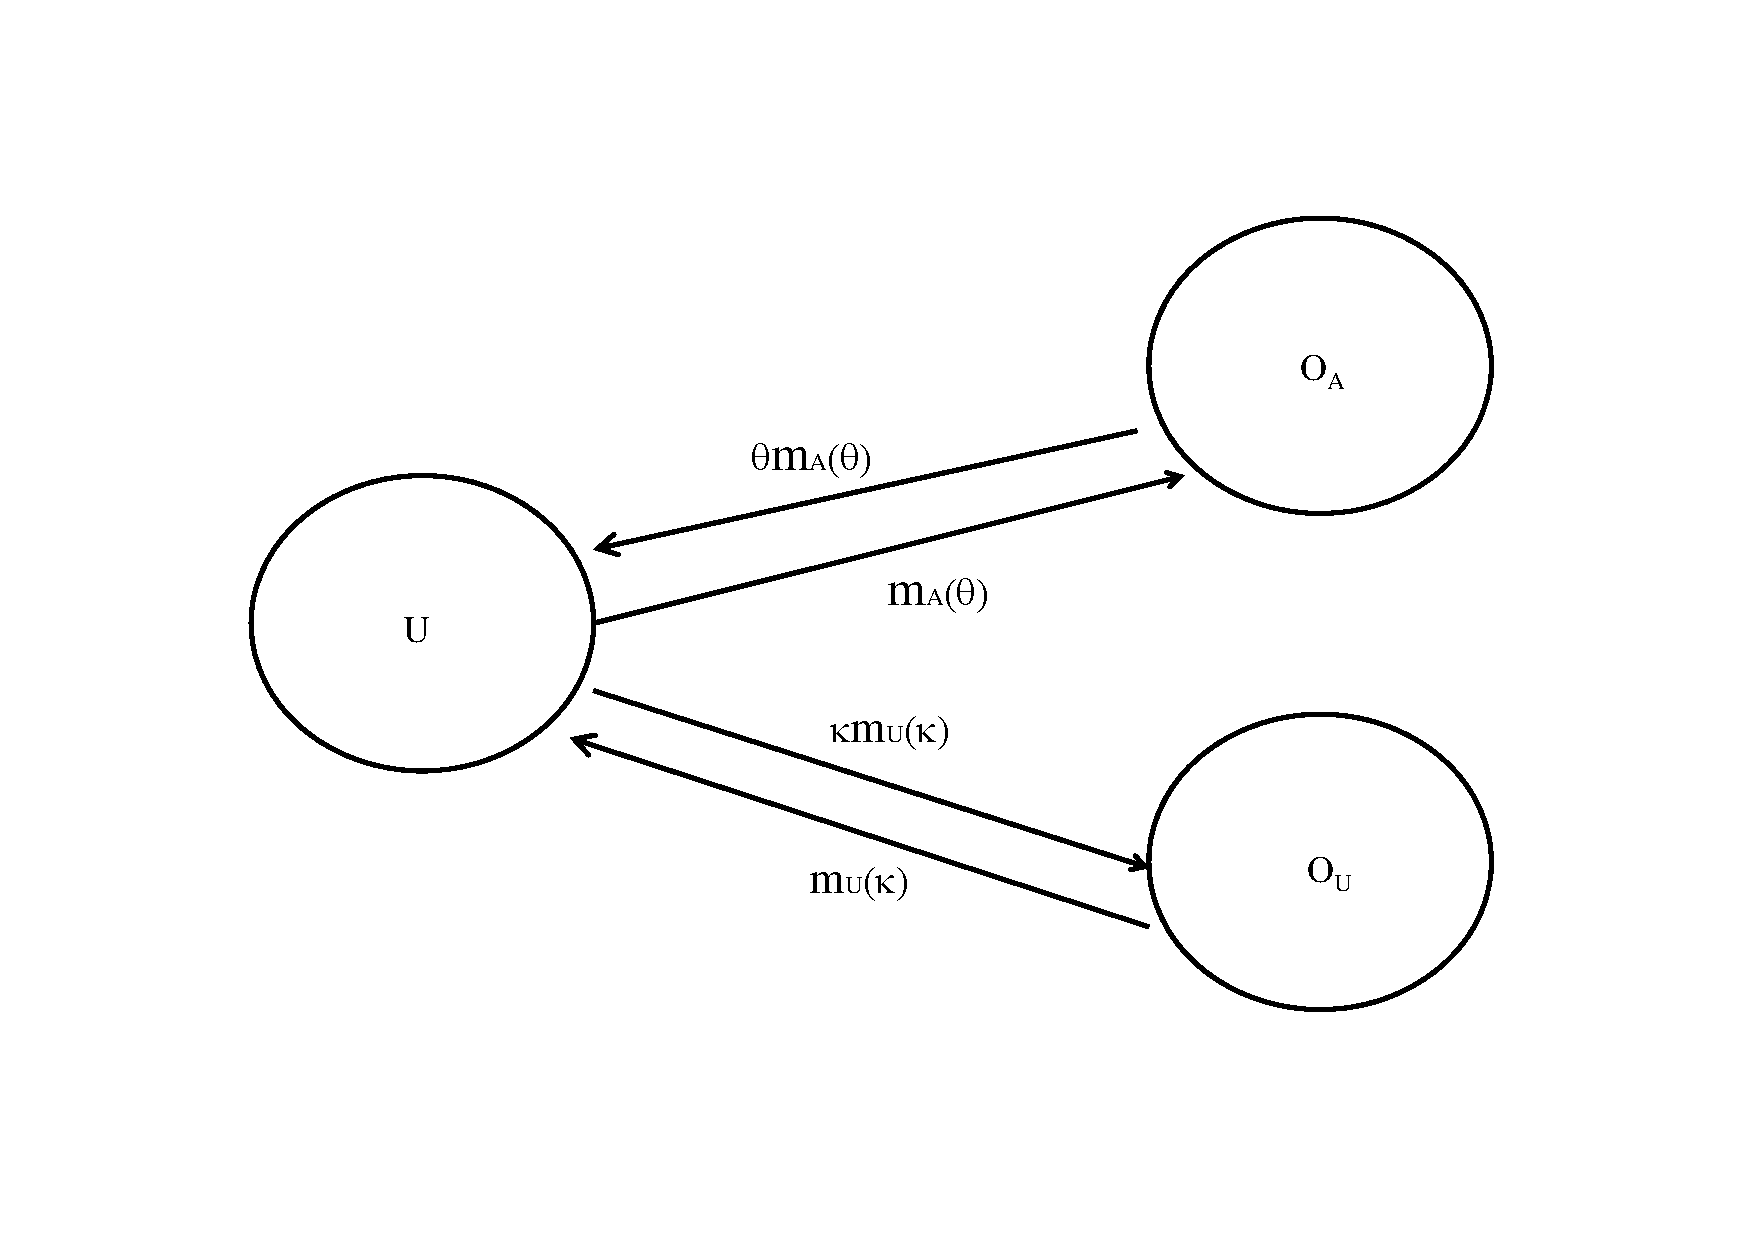
\includegraphics[width=\textwidth]{figures/flow_illustration.pdf}
\caption{Illustration of flows in the model}
\end{figure}

\subsubsection{Workers}

Let us proceed to describe the value functions of employed and unemployed workers, $V_e$ and $V_u$. When employed the worker enjoys a real wage of $w$, while loosing the job with an exogenous rate $q$. Thus, we can write the value function of being employed as
\begin{align}
r V_e= w+ q\left( V_u-V_e \right) 
\label{eq:rVe}
\end{align}

When unemployed the worker receives unemployment benefits of $z$, while matching into a job with probability $\theta m_A \left( \theta \right)+\kappa m_A \left( \kappa \right)$. Therefore, the value function of being unemployed reads
\begin{align}
r V_u= z+ \left[  \theta m_A \left( \theta \right)+\kappa m_A \left( \kappa \right) \right] \left( V_u-V_e \right) 
\label{eq:rVu}
\end{align}

\subsubsection{Firms}
\label{model:firm}

The value of a filled position depends on the firm's income stream from the position (productivity minus wage) plus the expected net loss from the possibility of job destruction.
\begin{align}
r \Pi_e=y-w+q \left( \Pi_{A/U}-\Pi_e \right)
\label{eq:rPie}
\end{align}

The value of a posting and unposted job-opening, respectively, reads as below. 
\begin{align}
r \Pi_A= -C_a+ m_A \left( \theta \right) \left( \Pi_E - \Pi_A \right) \\
r \Pi_U= -C_u+ m_A \left( \theta \right) \left( \Pi_E - \Pi_U \right) 
\end{align}
 Here $C_a$ reflects the job-posting cost, while $C_u$ reflects the cost of recruiting via other channels.

Assuming that job-opening are created until there is no profit to gain from creating additional openings\footnote{The free entry condition holds} $(\Pi_U=\Pi_A=0)$ we get two labour demand curves.

\begin{align}
\frac{C_a}{m(\theta)}=\frac{C_u}{m(\kappa)}=\frac{y-w}{r+q}
\label{eq:labourdemand}
\end{align}

\subsubsection{Wage bargaining}
Wages are determined via usual Nash bargaining, why workers and firm split the surplus from the match via the usual Nash-bargaining solution.
\begin{align}
\beta \Pi_E =\left( 1 -\beta \right) \left( V_u - V_e \right)
\end{align}
Here $\beta$ is the bargaining strength of the worker.

\subsubsection{The Augmented Beveridge curve}
Finally, we can note that the dynamics of unemployed in this model will follow the following dynamics.
\begin{align}
\dot{U}=\dot{N}+qL-\left[ \theta m_A \left( \theta \right) +\kappa m_U \left( \kappa \right) \right] U
\end{align}
which in steady state relates the unemployment rate to both types of job-openings via an \emph{augmented Beveridge curve}. 
\begin{align}
u=\frac{n+q}{\theta m_A \left( \theta \right)+\kappa m_A \left( \kappa \right)+n+q}
\end{align}

While the standard Beveridge curve is an object in two dimensions $(u, o)$, this augmented Beveridge curve is an object in three dimensions $(u, o_a, o_u)$. This also mean that the object often measured in data $(u, o_a)$ is merely a \emph{perceived} Beveridge curve. As we will illustrate below this opens up for alternative channels through which the perceived Beveridge curve can shift.

\begin{figure}
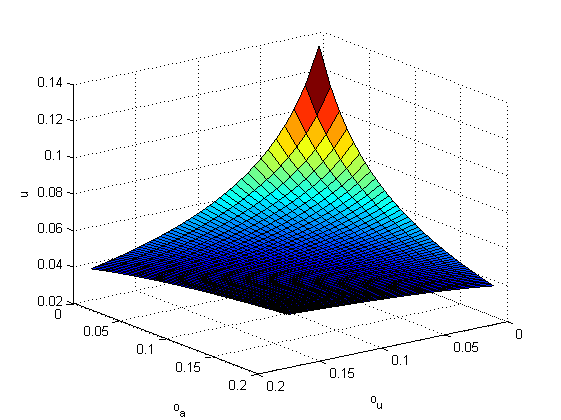
\includegraphics[width=\textwidth]{figures/BC_noeq}
\caption{The threedimentional Beveridge Curve.}
\end{figure}

\subsubsection{Equilibrium}
In sum, the equilibrium of our model is described by 6 equations with 6 unknown variables.


\begin{align}
u&=\frac{n+q}{\theta m_A \left( \theta \right)+\kappa m_A \left( \kappa \right)+n+q} \label{eq:eq_BC}\\
\frac{C_a}{m(\theta)}&=\frac{C_u}{m(\kappa)}=\frac{y-w}{r+q} \label{eq:eq_ld} \\
w&=\beta y + r(1-\beta)V_u \label{eq:eq_wage} \\
V_e-V_u&=\frac{\beta}{1-\beta}\frac{y-w}{r+q}=\frac{w-z}{\theta m_A \left( \theta \right)+\kappa m_A \left( \kappa \right)+r+q} \label{eq:eq_Ve_Vu}
\end{align}

\subsection{Mechanisms}

The relative cost of announced job openings is a key variable in the model. An increase in the cost of announced to unannounced openings will induce firms to shift their recruitment efforts from the announced to the unannounced market. This will lead to the share of announced openings and hires being decreasing in $C_a/C_u$ as illustrated in Figure \ref{fig:shares}. 

The relative cost of announced job openings will also impact on the perceived matching efficiency. 
Figure \ref{fig:perceived_BC} shows how the perceived Beveridge curve shifts inwards in response to an increase in the relative cost of announced job openings as firms respond to the higher cost of job announced openings by recruiting relatively more in the unannounced market. This will lower the ratio of announced job openings to unemployed which displays the inwards shift in the Beveridge curve. Similary, the perceived matching efficiency will increase when the relative cost of announced openings increases.

%The same mechanism in illustrated in Table \ref{tab:perceived_A}, where the impact of an increase in the relative cost of annonced openings on the \emph{perceived} matching efficiency is illustrated. 

What are the takeaway from this simple numerical exercise? First, the introduction of two recruitment channels, one announced and one unannonced, causes the \emph{Beveridge curve} to be an object in three dimensions $(u, o_a, o_u)$. Second, the two dimentional object often measured in data is merely a \emph{perceived} Beveridge curve. Third, the change in the cost of posting announced job-openings, which in the standard model leads to movements along the Beveridge curve, can in this augmented model shift the perceived matching efficiency and thus the Beveridge curve. 
These observations motivates the importance of accounting for the share of announced and unannounced job openings when analysing the labor market. 

%\begin{table}[htbp]
%\caption{Estimated matching function, $\log(h)=A+\alpha u+(1-\alpha) o$}
%\label{tab:perceived_A}
%\begin{tabularx}{\textwidth}{cXcXcXc}
 %\hline
  %$\lambda$ &  & A      &  & $\alpha$ &  & $1-\alpha$   \\
  %\hline 
  %\multicolumn{7}{c}{With $o=$ announced openings} \\
  %\hline 
  %$C_a=1.0$ &  & $0.69$ &  & $.50$    &  & $.50$    \\
  %$C_a=1.2$ &  & $0.74$ &  & $.50$    &  & $.50$          \\
 %\hline 
  %\multicolumn{7}{c}{With $o=$ total openings} \\
  %\hline
  %$C_a=1.0$ &  & $0.34$ &  & $.50$    &  & $.50$    \\
  %$C_a=1.2$ &  & $0.34$ &  & $.50$    &  & $.50$          \\
  %\hline 
%\end{tabularx}
%\end{table}

\begin{figure}[h!]
	\subfloat[Shares of announced positions and hires as function of the cost of posting announced job openings. \label{fig:shares}]{\includegraphics[width=.49\linewidth]{../Model/programs/WP_version/shares.png}}
	\subfloat[Perceived Beveridge Curve for two values of announcing job openings \label{fig:perceived_BC}]{\includegraphics[width=.49\linewidth]{../Model/programs/WP_version/BC.png}}
	\caption{Numerical illustrations}
	\label{fig:numeric}
\end{figure}


\subsection{Calibrating the Model}
\label{sec:Cali}

We will now use the data from section \ref{sec:Data} to calibrate the key parameters in the model laid out above.  Our calibration is shown in Table \ref{tab:calibration_full}. The elasticity of the matching function, $\alpha$, is obtained by estimating the matching function for announced openings. The bargaining power $\beta$ is sat such that the Hosios condition holds. The relative cost of job openings, $C_a/C_u$, is calibrated such that the model matches the share of hires via unannounced openings observed in the data. The level of $C_a$ is chosen so as to match a monthly job-finding probability of $0.20$. The value of unemployment benefits is sat to match a net replacement rate of 0.5. Finally, the job destruction rate and real interest rate are sat to $0.15$ and $0.05$, respectively.

\begin{table}[htbp]
\caption{Calibration}
\label{tab:calibration_full}
\begin{tabularx}{\textwidth}{cXcXl}
 \hline
  Parameter & & Value & & Source / Calibration  \\ 
  \hline 
   $y$ & & $10$   & & Normalisation    \\ 
   $r$ & & $.05$ & &             \\ 
   $q$ & & $.15$ & &            \\ 
   $z$ & & $4.8$   & & Replacement rate=0.5       \\ 
   $\beta$ & & $.8$ & & Hosios condition                 \\ 
	 $\alpha$ & & $.8$ & & Estimated matching function \\ 
	 $A_a=A_u$ & & $1$    & &  Normalisation              \\ 
	 %$A_u$ & & $1$    & &  Normalisation             \\ 
	 $C_u$ & & $.87$   & & Monthly job-finding rate=0.2               \\ 
	 $C_a/C_u$ & & $[1.73, 1.41]$   & & Share of unannounced hires $\in (0.90, 0.80)$               \\ 
  \hline
\end{tabularx}
\end{table}


\subsection{How much does the share of unannounced openings vary?}
We can now use the model and the data to adress our first question: how much does the share of unannounced job openings vary across time? Indeed, if we let $\mu_t$ be the share of hires made through unannounced openings (Figure \ref{fig:hires}) we can use the model to get the following expression for the share of unannounced job openings.\footnote{See appendicx \ref{app:CaCu} for derivation}
\begin{align}
\frac{O_u}{O_{a,}}=\left( \frac{1-\mu_t}{\mu_t} \right)^{\frac{1}{1-\alpha}}
\end{align}
Using this expression on the data we can plot the time series for the stock of unannounced openings and the share of unannounced openings as a ratio of total (Figure \ref{fig:openings_abs} and \ref{fig:openings_shares}). Some observations can be made from these two figures: (i) Unannounced openings accounts for the majority of job openings and (ii) during the recession (2008-09) the stock of these openings fell by much less than announced openings, (iii) the markets share of unannounced openings vary substantially over the business cycle. Taken together this indicates that announced openings only accounts for a small share and of all openings and that the share varies substantially across time.


\begin{figure}[h!]
	\subfloat[Job openings \label{fig:openings_abs}]{\includegraphics[width=.49\linewidth]{../Model/figures/openings}}
	\subfloat[Shares \label{fig:openings_shares}]{\includegraphics[width=.49\linewidth]{../Model/figures/openings_shares}}
	\caption{Announced and unannounced openings}
	%\label{fig:numeric}
\end{figure}


\subsection{What are consequences of swings in market shares for labor market analysis?}

To address this question we will assess what happens to the matching efficiency when the share of unannounced hires increases from 75 to 90 percent as was observed from 2008 to 2010. Specifically, we will calibrate $C_a/C_u$ so as to achieve these shares, and assess how the perceived matching efficiency differs across these two calibrated models.
%One where the share of announced hires takes the value of 0.95 (upper bound from data) and one where the shared of announced hires takes the value of 0.75 (lower bound from data). To achieve these shares we will set $C_a/C_u$ equal to $1.73$ and $1.41$, respectively.

Table \ref{fig:perceived_BC_high_low_cA} shows the result. An increase in the share of unannounced hires from $80$ to $90$ percent will, in the given calibration, increase the perceived matching efficiency by approx. 40 percent. Clearly, here the reason is not that the actual matching efficiency has gone up. Instead, it is simply a consequence of a drop in the share of announced openings caused by the higher posting costs. The table also illustrates that the seperate estimation of the two mathing function, obviously, is robust to fluctuations in the job posting costs. The similar mechanism is illustrated in Figure \ref{fig:perceived_BC_high_low_cA}. Here we show that the increase the share of unannounced openings causes an outwards shift in the Beveridge curve.

% we show the perceived Beveridge curve for a high and low value of $C_a/C_u$ consistent with the data. The figure shows how an increase in the relative cost of announced job-openings will shift the Beveridge curve inwards as the market share of announced openings decreases.

%Table \ref{fig:perceived_BC_high_low_cA} shows how the perceived matching efficiency is affected by the changes in the relative posting costs $(C_a/C_u)$ consistent with the data. The table shows the estimated matching efficiency on simulated data for upper and lower bounds for the relative posting consistent with the data. We see that an increase in the relative posting costs leads to an increase in the perceived matching efficiency. However, here the reason is not that the actual matching efficiency has gone up. Instead, it is simply a consequence of a drop in the share of announced openings caused by the higher posting costs. The table also illustrate that the seperate estimation of the two mathing function, obviously, is robust to fluctuations in the job posting costs.


\begin{figure}[p!]
\includegraphics[width=\textwidth]{../Model/programs/WP_version/BC_high_low_cA.png}
\caption{Perceived Beveridge Curve for $C_a/C_u \in \left\{ 1.41, 1.73 \right\}$.}
\label{fig:perceived_BC_high_low_cA}
\end{figure}

\begin{table}[htbp]
\caption{Estimated matching function, $\log(h)=A+\alpha u+(1-\alpha) o$}
\label{tab:perceived_A}
\begin{tabularx}{\textwidth}{cXcXcXc}
 \hline
  $ $ & & A & & $\alpha$ & & $1-\alpha$   \\ 
  \hline 
  & &  \multicolumn{5}{c}{$h=$ total hires, $o=$ announced openings} \\
  \hline 
   $C_a/C_u=1.41$ & & $2.07$ & &  $.8$ & & $.2$    \\ 
   $C_a/C_u=1.71$  & & $2.89$ & &  $.8$ & & $.2$          \\ 
 \hline 
   & &  \multicolumn{5}{c}{$h=$ announced hires, $o=$ announced openings} \\
	   $C_a/C_u=1.41$ & & $0$ & &  $.8$ & & $.2$    \\ 
   $C_a/C_u=1.71$  & & $0$ & &  $.8$ & & $.2$          \\ 
  \hline 
 & &  \multicolumn{5}{c}{$h=$ unannounced hires, $o=$ unannounced openings} \\
	   $C_a/C_u=1.41$ & & $0$ & &  $.8$ & & $.2$    \\ 
   $C_a/C_u=1.71$  & & $0$ & &  $.8$ & & $.2$          \\ 
\end{tabularx}
\end{table}


%\subsection{Robustness}
%
%\begin{itemize}
  %\item Composition
	%\item Model parameters.
	%\item Model formulation. No-arbitrage in search.
%%\end{itemize}

%\section{Matching functions}

\section{Concluding remarks}
\label{sec:conclusion}

This paper provides new evidence on firms recruiting behaviour. We create a new firm-level data set on  job-openings and hires in Denmark and show that only 10-25 percent of all hires are made through announced job-openings. Using a simple model we translate this into 5-20 percent of all job openings being announced. 
We also find considerable degree of variation across firm characteristics. The use of announced job openings is increasing in firm size, decreasing in employment growth and less used in start-ups than in existing firms. Moreover, the use of announced job openings exhibits an inverse u-shape in the firm's average wage level, with low- and high-wage firms relying the least on announced job openings. Accounting for swings in the use of announced job openings is important insofar that a decrease(increase) in the use of announced job-openings will cause a increase(decrease) in the perceived matching efficiency. Indeed, in our calibrated model a decrease in the use of announced job-openings from 20 to 10 percent (as observed in 2008-09) will increase the perceived matching efficiency by approx. 40 percent.

Important aspect are still work in progress. First, we need to understand the role of compositional changes across firms in the observed time variation in the share of announced hirings. Second, we have not yet exploited the worker dimension of our hiring data in order to understand how hiring channels differ across  observables on the individual level. Third, we need to understand  how our measure for job-openings relates to more all-encompassing surveys such as the JOLTS. 

\newpage

\section{Appendix}

\subsection{Solution Algoritm}
\label{sec:solution_algoritm}

First note that (\ref{eq:eq_ld}) can be used to find a $\kappa(\theta)$

\begin{align}
\kappa = \left( \frac{A_u/C_u}{A_a/C_a}\right)^{1/\alpha}
\end{align}

Then note that \ref{eq:eq_ld} also yields $w(\theta)$

\begin{align}
w(\theta)=y-\frac{\theta^\alpha (r+q)}{A_a/C_a}
\end{align}

Using this along with (\ref{eq:eq_Ve_Vu}) we can then find $\theta$ by solving this function numerically.

\begin{align}
\frac{\beta}{1-\beta}\frac{y-w(\theta)}{r+q}=\frac{w(\theta)-z}{\theta m_A \left( \theta \right)+\kappa m_A \left( \kappa(\theta) \right)+r+q}
\end{align}

This procedure yields solutions for $\theta$, $\kappa$, $w$. By means of (\ref{eq:eq_BC}) we can then back out $u$.

%\subsection{Detailed description of data creation}

%\subsection{Robustness of jobnet data}


%\subsection{Estimating the matching function for announced openings}
%\label{app:est_match}
%We start by finding suitable parameters for the matching function of announced job openings. Doing a constrained OLS on the logged matching function (\ref{eq:M_A}) yields the parameters shown in Table \ref{tab:estimation}.


%\begin{table}[htbp]
%\caption{Estimation of annonced matching function}
%\label{tab:estimation}
%\begin{tabularx}{\textwidth}{cXcXc}
% \hline
%  Parameter & & Value   \\ 
%  \hline 
%   $a_a$ & & $-0.93$       \\ 
%   $\alpha$ & & $.8$             \\ 
%  \hline
%\end{tabularx}
%\end{table}

%TBD: How would matching function differ with data for total hires?

\subsection{Calibration of $C_a/C_u$}
\label{app:CaCu}

Let $\mu$ be share of announced hires observed in the data. Then, we can easily back out the corresponding fraction of unannounced to announced openings.
\begin{align}
\frac{M(U, O_A)}{M(U, O_A)+M(U, O_U)}=\mu \Rightarrow \frac{1}{1+\left(\frac{O_U}{O_A}\right)^{1-\alpha}}=\mu \Rightarrow \frac{O_u}{O_a}=\left( \frac{1-\mu}{\mu}  \right)^{\frac{1}{1-\alpha}}
\end{align}

From one of the model's equilibrium conditions (\ref{eq:eq_ld}) we know that this fraction can be written as a function of relative job posting costs.
\begin{align}
 \frac{C_a}{C_u}=\frac{m\left( \theta \right)}{m\left( \kappa \right)} \Rightarrow \frac{C_a}{C_u}=\left(\frac{O_u}{O_a} \right)^\alpha
\end{align}

Thus, $C_a/C_u$ can be calibrated as 
\begin{align}
\frac{C_a}{C_u}=\left( \frac{1-\mu}{\mu}  \right)^{\frac{\alpha}{1-\alpha}}
\end{align}


%\subsection{Calibrating the cost of job-openings}
%Using the data for announced and unannounced job-openings (Figure \ref{fig:openings}-\ref{fig:openings_shares}), we can now calibrate the costs parameters for job openings, $C_a$ and $C_u$. Specifically, we will set $C_u=1$\footnote{Consider a better calibration. Potentially to hit a certain average job finding rate.} and then calibrate $C_a$ so as to match the market share for unannounced job openings that we observe in the data (Figure \ref{fig:openings_shares}). As this share is varying over time we will calibrate $C_a$ for a range of market share. Table \ref{tab:cali_ca} shows how the calibration of $C_a$ depends on the market share of unannounced openings. To generate a higher market share of unannounced openings we need a higher cost of announced openings.
%
%\begin{table}[htbp]
%\caption{Calibration of $C_a$}
%\label{tab:cali_ca}
%\begin{tabularx}{\textwidth}{cXcX}
 %\hline
  %$\frac{O_u}{O_u+O_a}$ & & $C_a$  \\ 
  %\hline 
   %$0.80$ & & $3.03$   \\ 
	 %$0.85$ & & $4.00$   \\ 
	 %$0.90$ & & $5.84$   \\ 
 %\hline 
%\end{tabularx}
%\end{table}

%\subsection{Backing out the stock of unannounced openings}
%
%We will now use the model and data presented above to back out the stock of unannounced job openings. The data for hirings (Figure X) can be combined with the matching function in order to get a measure for the stock of unannounced openings. Indeed, using the matching function we can write the stock of unannounced openings\footnote{Small letters means variables in logs.}
%\begin{align}
%o_u=\frac{h_u-a_a-(1-\alpha)u}{\alpha}
%\label{eq:ou}
%\end{align}
%$h_u$ and $u$ are directly from the data, while the parameters $\alpha$ and $a_u$ are taken from the section above. $a_a$ is uninteresting in the sense that it is only affect the level. On the other hand $\alpha$ can affect the time fluctuations, why we will conduct robustness check on the assumption $\alpha_a=\alpha_u$.
%
%Figure \ref{fig:openings} shows the resulting stock of both announced and unannounced openings. Figure \ref{fig:openings_shares} shows the implied market share of announced and unannounced job openings, respectively. Several interesting features stands out from these two figures: (i) Unannounced openings accounts for the vast majorities of all job openings ($75\%-95\%$) and (ii) during the 2008 recession  the stock of these openings fell by much less than announced openings, (iii) the markets share of unannounced openings vary substantially over the observed period. Taken together this indicates that announced openings only accounts for a small share and of all openings and that the share varies substantially across time.
%
%\begin{center}
	%
%[Insert empirical BC]
%
%\end{center}


\bibliography{bib}
\end{document}